\makeatletter%
\special{pdf: put @thispage <</Group << /S /Transparency /I true /CS /DeviceRGB>> >>}%
\makeatother%
\documentclass[a4paper,twoside,10pt]{article}
\usepackage[left=2.45cm,top=2.52cm,right=1.85cm,bottom=2.95cm]{geometry}

\usepackage[xetex]{hyperref}

\usepackage{csquotes}

\usepackage{graphicx}

\usepackage[backend=biber,style=alphabetic,natbib=true]{biblatex}
\addbibresource{bibliography.bib}

\title{Notes to Andrew Ng's Machine Learning Course}
\author{Jan Wedekind}

\begin{document}
\maketitle

\section{Introduction}

\subsection{What is Machine Learning}
These are course notes to Andrew Ng's video lecture\citep{andrewng}. A well-posed learning problem (as defined by Tom Mitchell) is:
\begin{displayquote}
  A computer program is said to \emph{learn} from experience E with respect to some task T and some performance measure P, if its performance on T, as measured by P, improves with experience E.
\end{displayquote}

\subsection{Supervised Learning}
\begin{figure}[htbp]
  \begin{center}
    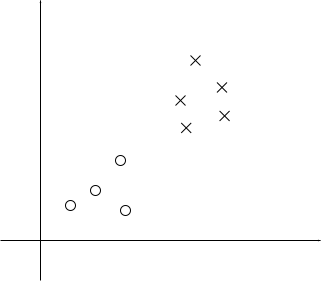
\includegraphics[width=.4\textwidth]{supervised}
  \end{center}
  \caption{Labelled data for supervised learning\label{fig:supervised}}
\end{figure}
Two examples for problems of different learning problems (given labelled data as shown in Figure \ref{fig:supervised}) are given
\begin{itemize}
  \item Regression problem (continuous value): estimating house price given size in square feet
  \item Classification problem (discrete values): determine whether a tumor is malignant or benign given size of tumor and age of person
\end{itemize}

\subsection{Unsupervised Learning}
\begin{figure}[htbp]
  \begin{center}
    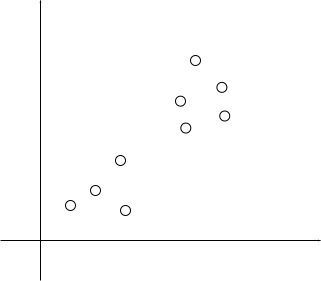
\includegraphics[width=.4\textwidth]{unsupervised}
  \end{center}
  \caption{Data without labels\label{fig:unsupervised}}
\end{figure}
When the data is not labelled (see Figure \ref{fig:unsupervised}), one can still apply clustering algorithms to it.
For example Google News clusters groups related news articles into stories.
Another basic but impressive example is separating two audio sources (speaker and a radio) using data from two microphones.

For development Andrew Ng recommends GNU Octave\citep{octave}.

\printbibliography

\end{document}
